\part{Stratégie de développement}
\section{Méthologie de développement}

\section{Intégration continue}
Afin de collaborer au mieux au sein de l'équipe, nous avons mis en place
une C.I. (Continious Integration). C'est un pipeline qui consiste à executer
les tests mis en places automatiquement après chaque changement sur une branche
du projet.

Après avoir positivement passé les tests et avoir subit une phase de review
pour recevoir commentaires et conseils, le code peut être intégré dans la
branche principale avec l'assurance (relative à l’exhaustivité des tests) qu'il
n'a rien cassé.

Cette méthodologie de travail permet à l’utilisateur final de récuperer toutes
les nouveautés introduites au moment où elles sont \emph{merged} et non à la
sortie d’une nouvelle version. Dans certain cas, notamment avec les sites web
par exemple, on peut même arriver à faire du Continuous Deployment, ce qui veut
dire qu’il n’y a plus besoin de versionner les différents états du projet et
qu’à chaque push d’un des développeur, le site disponible à l’utilisateur est
celui contenant le dernier commit. Ceci n'est pas possible à faire pour un
projet comme le notre, qui doit être manuellement mis-à-jour à chaque nouvelle
version.
\\
\\
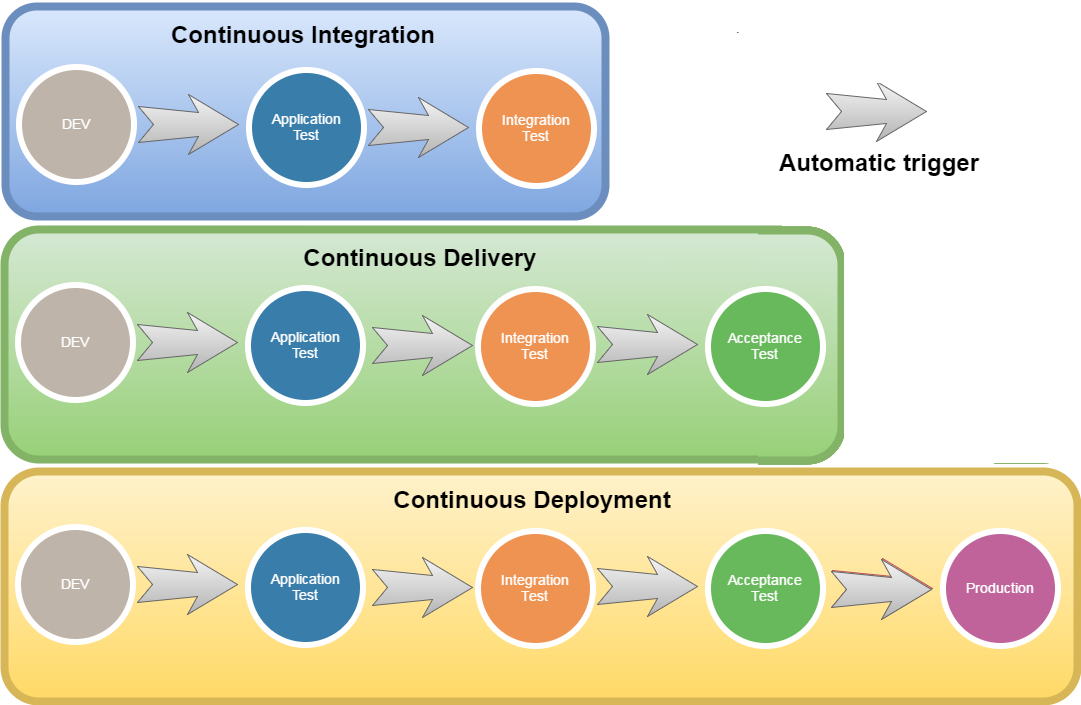
\includegraphics[width=\linewidth]{CI-CD}
